\documentclass[10pt,twocolumn]{article}

\usepackage[a4paper,margin=1.7cm]{geometry}
\usepackage{kotex}
\usepackage{amsmath,amssymb}
\usepackage{graphicx}
\usepackage{booktabs}
\usepackage{caption}
\usepackage{hyperref}
\usepackage{enumitem}

\graphicspath{{figures/}{./}}
\setlist[itemize]{leftmargin=1.2em}
\setlength{\columnsep}{0.7cm}
\captionsetup{font=small}
\renewcommand{\arraystretch}{1.15}

\title{\textbf{FedLoG 기반 실험 환경에서의 노드 특징 그래디언트 역추론 분석}\\
\large GNN 연합학습의 제한적 위협 모델과 방어 비교}
\author{진로 탐색 프로젝트}
\date{2026}

\begin{document}
\maketitle

\begin{abstract}
연합학습(Federated Learning, FL)은 원본 데이터를 중앙 서버에 보내지 않는다는 점에서 프라이버시 친화적 학습 방식으로 여겨진다. 그러나 클라이언트가 공유한 그래디언트나 모델 업데이트만으로도 원본 입력을 추정할 수 있는 DLG(Deep Leakage from Gradients) 계열 공격이 알려지며 이러한 가정은 더 이상 충분하지 않다. 본 연구는 FedLoG\cite{kim2025fedlog}의 전체 성능 재현이나 정식 프라이버시 보장을 목표로 하지 않고, FedLoG의 2-layer GraphSAGE와 합성 노드/특징 변환 식을 활용한 제한적 실험 환경에서 개별 클라이언트 업데이트가 노드 특징을 얼마나 노출하는지 분석한다. 공격자는 모델, 손실 함수, 그래프 구조와 관찰 대상 업데이트를 알고 있으며, 타겟 노드 또는 작은 배치의 특징 벡터를 그래디언트 매칭으로 복원한다고 가정하였다. WikiCS 기반 초기 실험($n=5$)은 복원도가 시드와 타겟 노드에 크게 의존함을 보였고, Cora 공식 분할 기반 재검증($n=10$)에서는 batch size 1에서 무방어 복원 코사인이 $0.754 \pm 0.123$, FedLoG 특징 변환 포함 조건이 $0.773 \pm 0.116$으로 큰 차이를 보이지 않았다. 반면 90--95\% 희소화는 복원 코사인을 $0.014$--$0.028$ 수준으로 낮췄다. 가우시안 노이즈 교란은 강도에 따라 복원을 낮췄지만 정식 $(\varepsilon,\delta)$-차분 프라이버시 분석은 수행하지 않았으므로, 본문에서는 이를 DP-inspired 그래디언트 교란으로만 부른다. 결과는 GNN 기반 FL에서도 제한된 조건에서 노드 특징 유출 가능성이 있음을 보이지만, 그래프 구조 전체 복원이나 일반적 FedLoG 안전성에 대한 결론으로 확대해서는 안 된다.
\end{abstract}

\noindent\textbf{주요어:} 연합학습, 그래프 신경망, FedLoG, 그래디언트 유출, DLG, 희소화, DP-inspired 그래디언트 교란

\section{서론}
연합학습은 각 클라이언트가 원본 데이터를 보관한 채 로컬 학습 결과만 서버와 공유하는 분산 학습 방식이다. 하지만 원본 데이터가 직접 전송되지 않는다는 사실만으로 프라이버시가 보장되지는 않는다. Zhu 등\cite{zhu2019dlg}은 공유 그래디언트만으로 입력 데이터를 복원하는 DLG 공격을 제안했고, 이후 iDLG\cite{zhao2020idlg}와 Inverting Gradients\cite{geiping2020inverting}는 라벨 추론과 코사인 기반 그래디언트 매칭을 통해 공격 안정성을 높였다.

이미지 모델에 대한 그래디언트 역추론은 비교적 많이 연구되었지만, 그래프 신경망(GNN)의 연합학습에서는 노드 특징과 그래프 구조, 메시지 패싱이 함께 얽혀 있어 위협 모델을 더 조심스럽게 정의해야 한다. 최근 GraphDLG\cite{wei2026graphdlg}처럼 그래프 구조와 노드 특징의 결합 복원을 직접 다루는 연구도 등장했으나, 본 연구의 범위는 그보다 좁다. 즉, 그래프 구조와 학습 조건을 알고 있는 서버가 개별 클라이언트의 단일 로컬 업데이트 또는 이에 준하는 그래디언트를 관찰할 때, 특정 노드 특징 벡터가 얼마나 복원되는지를 실험적으로 확인한다.

본 연구의 기여는 다음과 같다.
\begin{itemize}
\item FedLoG 기반 GraphSAGE 실험 환경에서 노드 특징 그래디언트 역추론 공격을 구현하였다.
\item FedLoG 원 논문이 프라이버시 방어를 주장한다고 해석하지 않고, 합성 노드와 특징 변환을 포함한 조건이 유출을 줄이는지 별도 실험으로 검증하였다.
\item 시드 고정이 없는 단일 실행 보고의 위험성을 보이고, Cora 공식 분할 기반 $n=10$ 재검증을 추가하였다.
\item 희소화와 가우시안 노이즈 교란을 기존 방어/압축 기법의 비교 대상으로 적용하되, 정식 DP 보장이나 새로운 방어 기법으로 과장하지 않는다.
\end{itemize}

\section{연구 배경}
\subsection{FedAvg와 그래디언트 유출}
전형적인 FedAvg\cite{mcmahan2017fedavg}에서는 클라이언트가 여러 로컬 스텝을 수행한 뒤 모델 파라미터 또는 업데이트량을 서버에 보내고, 서버는 이를 평균해 전역 모델을 갱신한다. 따라서 모든 FedAvg 구현이 원시 미니배치 그래디언트를 직접 전송한다고 볼 수는 없다. 본 연구의 위협 모델은 더 제한적이다. 악의적 서버가 secure aggregation 없이 개별 클라이언트의 단일 로컬 스텝 그래디언트 또는 그와 매우 가까운 업데이트를 관찰할 수 있다고 가정한다.

DLG 공격은 더미 입력 $x'$를 초기화한 뒤 더미 입력이 만드는 그래디언트와 관찰 그래디언트의 차이를 줄이는 최적화 문제로 표현된다. 이미지에서는 TV 정규화가 복원 품질을 안정화하지만, 그래프의 희소 특징 벡터에는 적절하지 않으므로 본 연구에서는 코사인 그래디언트 손실과 약한 $L_2$ 정규화를 사용하였다.

\subsection{FedLoG와 본 연구의 해석 범위}
FedLoG\cite{kim2025fedlog}는 서브그래프 연합학습에서 local generalization을 개선하기 위한 방법이다. 핵심 목적은 프라이버시 방어가 아니라, 로컬 데이터에 부족한 클래스/구조 정보를 합성 노드와 지식 응축으로 보완하는 것이다. 따라서 본 논문은 FedLoG를 ``프라이버시 방어 모델''로 서술하지 않는다. 대신 FedLoG 식에서 사용하는 합성 특징과 특징 변환을 포함한 학습 조건이 그래디언트 유출 관점에서 어떤 영향을 주는지 별도로 측정한다.

\section{실험 방법}
\subsection{위협 모델}
공격자는 서버이며, 모델 구조와 현재 파라미터, 손실 함수, 그래프 구조, 타겟 배치의 라벨을 알고 있다고 가정한다. 공격자는 집계 전 타겟 클라이언트의 업데이트를 관찰한다. 복원 대상은 전체 그래프가 아니라 타겟 노드 또는 작은 배치의 노드 특징이다. 이웃 노드와 adjacency가 알려져 있으므로, 본 설정은 그래프 구조와 특징을 동시에 복원하는 공격보다 쉽고 제한적이다.

\subsection{구현과 설정}
공식 FedLoG Cora 분할(`data/FedLoG/closeset/Cora/4/local_graphs.pkl`)을 사용했고, 모델은 2-layer GraphSAGE 인코더와 선형 분류기로 구성하였다. 합성 노드는 클래스별 로컬 평균 특징을 class-rate로 가중 집계한 CPU 재현이며, FedLoG 전체 condensation 파이프라인을 완전 재현한 것은 아니다. 학습은 30라운드, hidden dimension 32, SGD형 FedAvg 업데이트 학습률 0.05로 수행하였다. 공격은 Adam(lr 0.12), 200 iterations, batch size 1과 4에서 수행하였다. 환경은 Python 3.10.20, PyTorch 2.0.1, PyG 2.4.0, CPU 실행이다.

비교 조건은 무방어(plain), 합성 특징 포함 순진 공격(fedlog\_naive), 특징 변환 파라미터까지 추정하는 적응형 공격(fedlog\_adaptive), 가우시안 노이즈 교란(noise 0.0001/0.001), 90\%와 95\% 희소화이다. 여기서 noise 조건은 DP-SGD에서 쓰이는 클리핑과 가우시안 노이즈의 아이디어를 차용했지만, 보호 단위, 인접 데이터셋, privacy accountant, 최종 $(\varepsilon,\delta)$를 계산하지 않았으므로 정식 차분 프라이버시 보장으로 주장하지 않는다.

\section{실험 결과}
\subsection{초기 WikiCS 실험의 한계}
기존 WikiCS 기반 초기 실험($n=5$)에서는 무방어 평균 복원 코사인이 $0.384 \pm 0.316$, FedLoG 특징 스케일링 조건이 $0.385 \pm 0.447$, 적응형 공격 조건이 $0.852 \pm 0.174$였다. 이 결과는 난독화가 안정적 방어로 보기 어렵다는 신호를 주지만, 표준편차가 매우 크고 target/seed 정의가 결과에 크게 영향을 준다. 또한 시드 미고정 원본 실행 5회에서 나온 0.518--0.999 범위는 동일한 $n=5$ 평균과 직접 비교할 수 없는 별도 감사 결과이다. 따라서 본 논문은 이 수치를 확정 결론이 아니라 재검증 필요성을 보여주는 예비 결과로만 사용한다.

\begin{table}[t]
\caption{Cora 공식 분할 기반 FedLoG 식 재검증 결과($n=10$, 중복 제거)}
\label{tab:fedlog_required}
\centering
\footnotesize
\resizebox{\columnwidth}{!}{%
\begin{tabular}{lcccc}
\toprule
조건 & \multicolumn{2}{c}{batch 1} & \multicolumn{2}{c}{batch 4} \\
\cmidrule(lr){2-3}\cmidrule(lr){4-5}
 & 코사인 & NMSE & 코사인 & NMSE \\
\midrule
Plain & $0.754\pm0.123$ & $0.8\pm0.6$ & $0.409\pm0.141$ & $1.7\pm0.7$ \\
FedLoG naive & $0.773\pm0.116$ & $0.8\pm0.6$ & $0.435\pm0.141$ & $1.7\pm0.7$ \\
FedLoG adaptive & $0.773\pm0.112$ & $0.7\pm0.5$ & $0.428\pm0.150$ & $1.6\pm0.6$ \\
Noise 0.0001 & $0.773\pm0.113$ & $0.7\pm0.5$ & $0.427\pm0.150$ & $1.6\pm0.6$ \\
Noise 0.001 & $0.734\pm0.123$ & $0.9\pm0.6$ & $0.309\pm0.087$ & $2.9\pm1.3$ \\
Sparse 90\% & $0.028\pm0.010$ & $1773.7\pm1055.4$ & $0.015\pm0.002$ & $3958.7\pm1778.0$ \\
Sparse 95\% & $0.019\pm0.006$ & $3986.9\pm2093.7$ & $0.014\pm0.003$ & $5371.9\pm2099.7$ \\
\bottomrule
\end{tabular}}
\end{table}

\subsection{Cora 재검증 결과}
표~\ref{tab:fedlog_required}와 그림~\ref{fig:fedlog_required}는 Cora 공식 분할에서 수행한 재검증 결과이다. batch size 1에서는 무방어 코사인이 $0.754 \pm 0.123$으로 높았고, FedLoG naive와 adaptive 조건도 각각 $0.773 \pm 0.116$, $0.773 \pm 0.112$로 거의 같았다. 이는 본 설정에서 합성 특징/특징 변환이 노드 특징 복원을 줄이지 못했음을 의미한다. batch size 4에서는 모든 비희소 조건의 코사인이 낮아졌지만, FedLoG 조건이 무방어보다 명확히 안전하다고 보기는 어렵다.

가우시안 노이즈 0.001은 batch size 4에서 코사인을 $0.309 \pm 0.087$로 낮췄지만, batch size 1에서는 $0.734 \pm 0.123$에 머물렀다. 더 강한 노이즈가 필요할 수 있으나, 그 경우 학습 유용성 손실도 함께 평가해야 한다. 90\%와 95\% 희소화는 두 batch size 모두에서 복원 코사인을 거의 0에 가깝게 낮췄다. 다만 희소화 결과의 gradient fidelity가 높게 나타나는 이유는 제거된 작은 좌표들이 원래 그래디언트 방향에 거의 기여하지 않았기 때문이며, NMSE는 크게 증가했다. 따라서 코사인과 NMSE를 함께 해석해야 한다.

\begin{figure}[t]
\centering
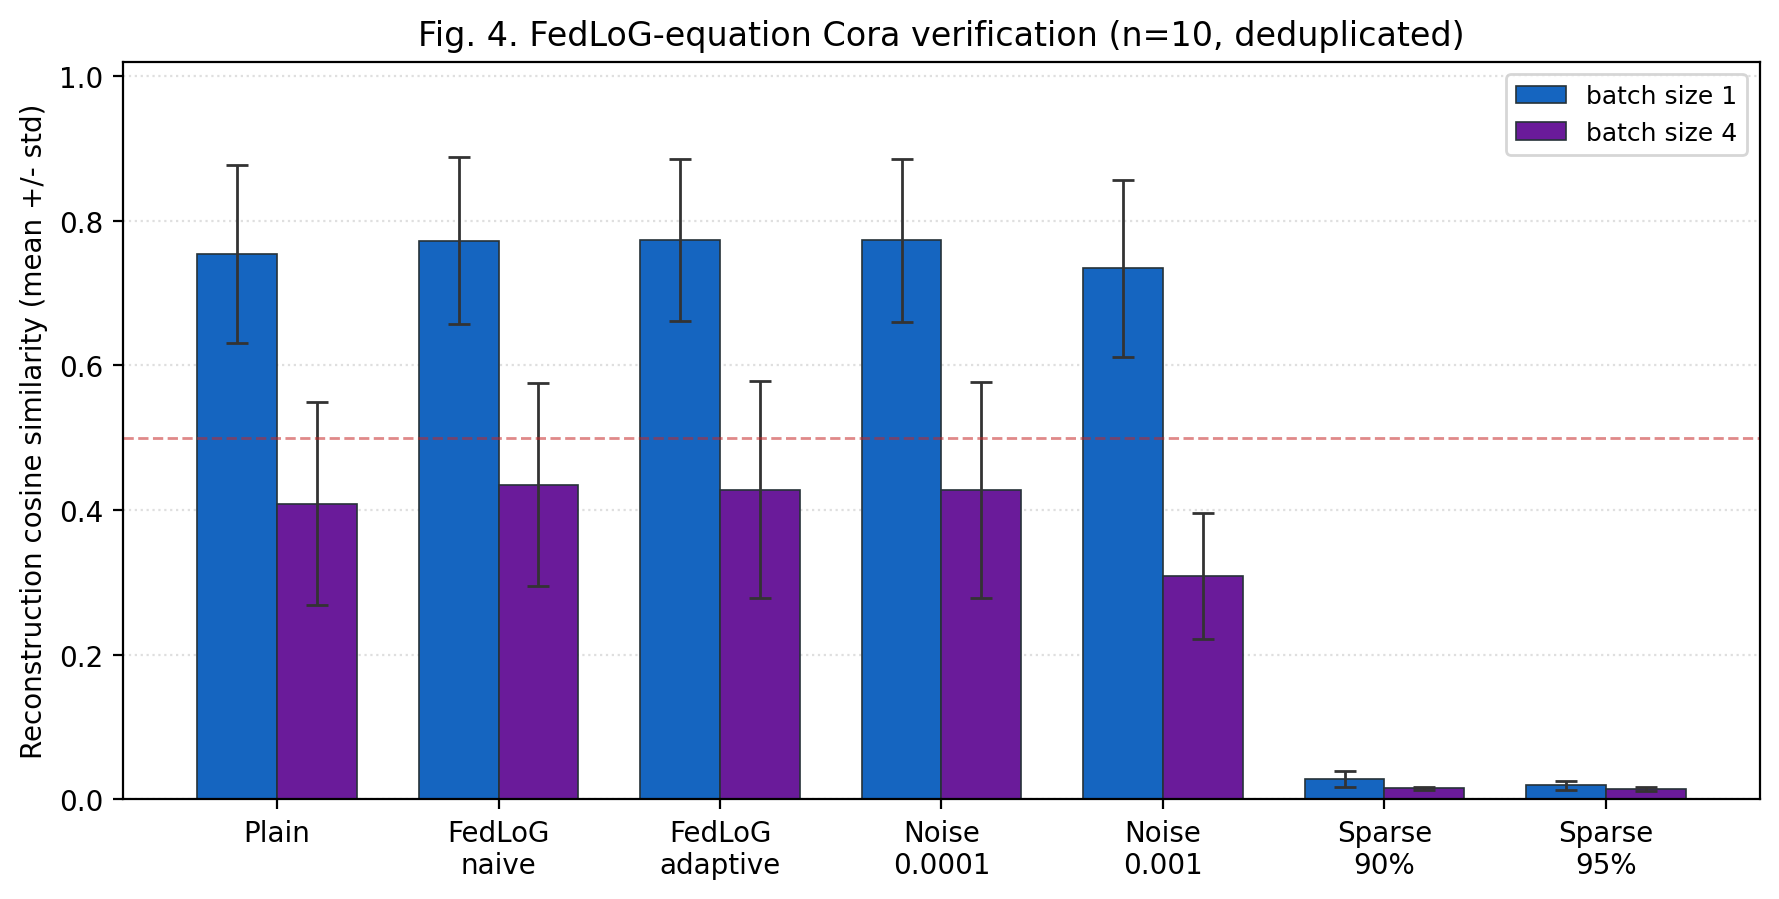
\includegraphics[width=\columnwidth]{fig4_fedlog_required.png}
\caption{Cora 공식 분할 기반 FedLoG 식 재검증의 복원 코사인}
\label{fig:fedlog_required}
\end{figure}

\subsection{실제 유용성 지표}
30라운드 학습 후 모든 조건의 테스트 정확도는 $0.305 \pm 0.000$, macro-F1은 $0.067 \pm 0.000$이었다. 이는 본 CPU 재현이 FedLoG의 local generalization 성능을 충분히 재현한 것이 아니라, 프라이버시 공격을 분리해 살피기 위한 제한적 실험 환경임을 보여준다. 따라서 본 연구의 ``유용성'' 결론은 실제 서비스 성능에 대한 결론이 아니라, 후속 실험에서 더 긴 학습, 공식 condensation, unseen/local generalization 지표가 필요하다는 근거로 해석해야 한다.

\section{논의}
첫째, 본 실험 범위에서는 FedLoG의 합성 특징과 특징 변환을 포함해도 노드 특징 역추론이 줄어든다고 보기 어려웠다. 이는 FedLoG가 원래 프라이버시 방어 논문이 아니라 local generalization 개선 논문이라는 점과도 일치한다. 둘째, 코사인 기반 역추론은 스케일 변화에 둔감하므로, 단순한 특징 스케일링을 프라이버시 방어로 해석하는 것은 위험하다. 셋째, 희소화는 본 설정에서 강한 복원 차단 효과를 보였지만, 이는 기존 압축/방어 기법의 적용 결과이지 새로운 방어 방법의 제안은 아니다.

한계도 분명하다. 본 연구는 Cora와 WikiCS 일부 설정, 2-layer GraphSAGE, 작은 batch size, 알려진 구조와 라벨, CPU 재현에 한정된다. GraphDLG\cite{wei2026graphdlg}처럼 구조와 특징을 동시에 복원하는 공격과 비교하지 않았고, 정식 privacy accounting도 수행하지 않았다. 따라서 결론은 ``FedLoG 기반 제한 실험 환경에서 노드 특징 유출 가능성이 확인되었다''로 제한해야 하며, GNN 기반 FL 전체 또는 FedLoG 원 모델 전체의 안전성에 대한 일반 결론으로 확장해서는 안 된다.

\section{결론}
본 연구는 FedLoG 기반 GraphSAGE 실험 환경에서 개별 클라이언트 업데이트가 노드 특징 정보를 노출할 수 있음을 확인하였다. Cora 공식 분할 기반 $n=10$ 재검증에서 무방어와 FedLoG 특징 변환 조건의 복원 코사인은 큰 차이를 보이지 않았고, 90--95\% 희소화는 복원을 강하게 낮췄다. 그러나 가우시안 노이즈 교란은 정식 DP 보장이 아니며, 본 CPU 재현의 학습 성능도 낮기 때문에 실제 프라이버시-유용성 절충을 결론짓기에는 부족하다. 향후에는 FedLoG 공식 condensation 파이프라인, 더 많은 target node와 seed, random/mean feature baseline, privacy accountant, 그리고 구조-특징 동시 복원 공격과의 비교가 필요하다.

\begin{thebibliography}{99}

\bibitem{mcmahan2017fedavg}
H. B. McMahan, E. Moore, D. Ramage, S. Hampson, and B. A. y Arcas, ``Communication-Efficient Learning of Deep Networks from Decentralized Data,'' in \textit{AISTATS}, 2017.

\bibitem{zhu2019dlg}
L. Zhu, Z. Liu, and S. Han, ``Deep Leakage from Gradients,'' in \textit{NeurIPS}, 2019.

\bibitem{zhao2020idlg}
B. Zhao, K. R. Mopuri, and H. Bilen, ``iDLG: Improved Deep Leakage from Gradients,'' \textit{arXiv preprint arXiv:2001.02610}, 2020.

\bibitem{geiping2020inverting}
J. Geiping, H. Bauermeister, H. Dr\"oge, and M. Moeller, ``Inverting Gradients: How Easy Is It to Break Privacy in Federated Learning?,'' in \textit{NeurIPS}, 2020.

\bibitem{abadi2016dp}
M. Abadi et al., ``Deep Learning with Differential Privacy,'' in \textit{CCS}, 2016.

\bibitem{kim2025fedlog}
S. Kim et al., ``Subgraph Federated Learning for Local Generalization,'' in \textit{ICLR}, 2025.

\bibitem{wei2026graphdlg}
S. Wei, W. Chen, T. Wei, C. Gong, Y. Tong, and L. Cui, ``GraphDLG: Exploring Deep Leakage from Gradients in Federated Graph Learning,'' \textit{arXiv preprint arXiv:2601.19745}, 2026.

\end{thebibliography}

\end{document}
